\subsection{Magnitude and Phase as Functions of Frequency}

Once the system was solved symbolically, the complex amplitudes in function of the frequency could be obtain symbol by keeping $t=0$, and varying only the frequency, which in this case was done in the interval between $0.1$ and $10^6$ Hz. This time the goal was specifically to get the magnitude and the phase, instead of the complex amplitude, so as before were used the norm and the argument.

\begin{figure}[H]
    \centering
    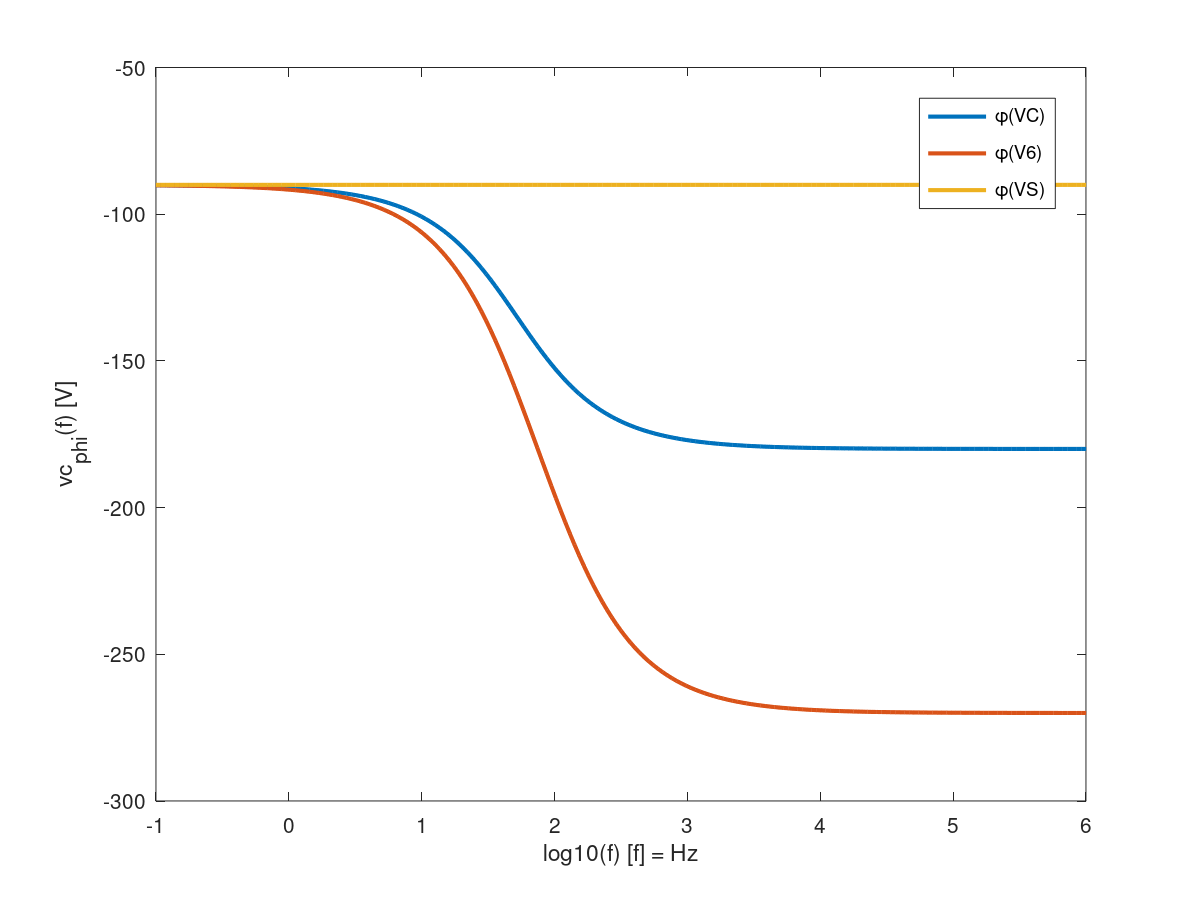
\includegraphics[width = 0.85\linewidth]{../mat/vcphi.png}
        \caption{\textit{Plot of the phase in function of the frequency. The frequency is presented in a logarithmic scale, contrary to the phase which is in linear scale in degrees.}}
    \label{fig:phase}
\end{figure}

As expected the phase for the voltage source is not dependent on the frequency, which was clear in the formula used to define it. More interestingly, the phase for both $V_c$ and $V_6$ seem to decrease around $50Hz$, stabilizing in a quarter and half a period, respectively, for higher frequencies.  


\begin{figure}[H]
    \centering
    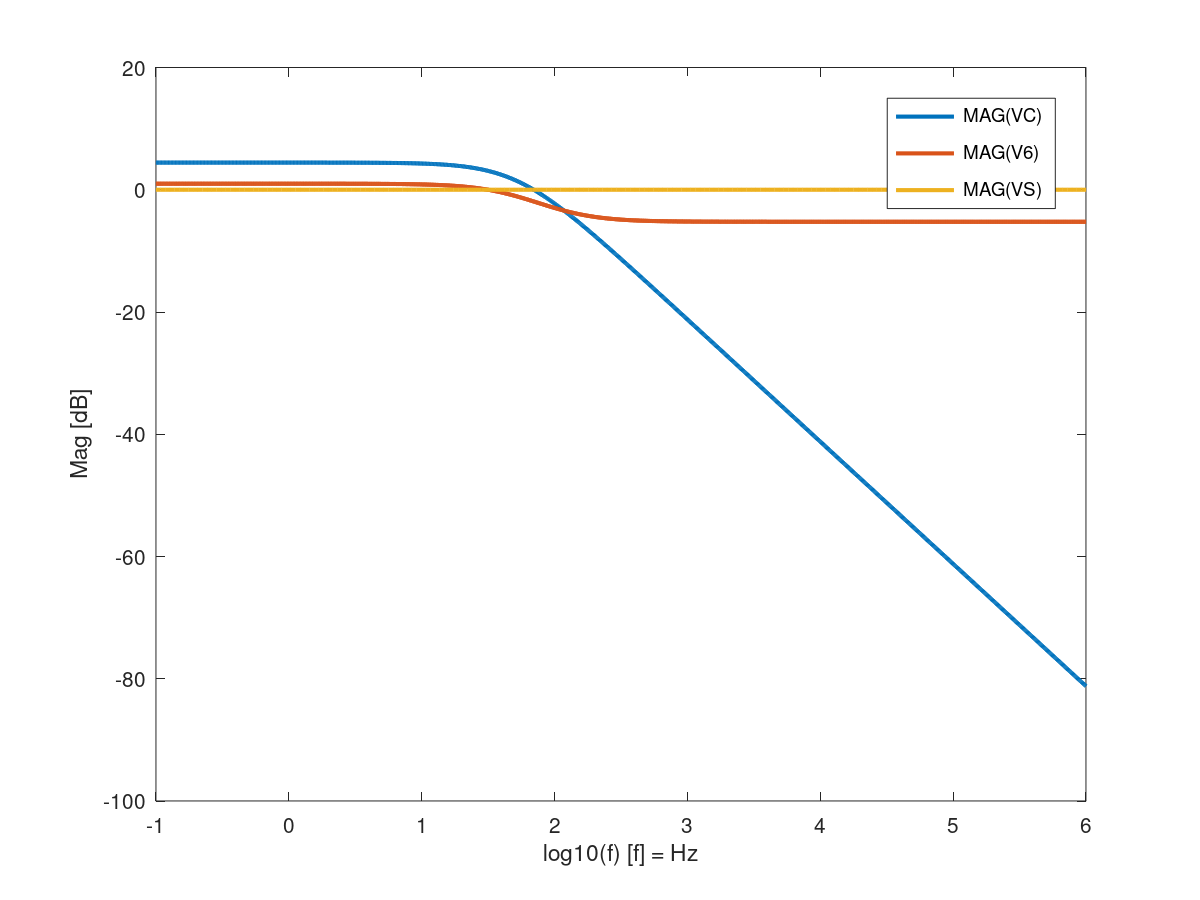
\includegraphics[width = 0.85\linewidth]{../mat/vcmag.png}
        \caption{\textit{Plot of the magnitude in function of the frequency. The frequency is presented in a logarithmic scale, as is the magnitude, which is in dB.}}
    \label{fig:magnitude}
\end{figure}

With amplitude $1$, $V_s$ has a constant magnitude for any frequency as expected, contrary to the other amplitudes that decrease with the increase in frequency, and for really high oscillation in the source, the amplitude of the oscillation in node 6 is practically 0. The critical frequency seems to be at $80Hz$.